% GNUPLOT: LaTeX picture with Postscript
\begingroup
  \makeatletter
  \providecommand\color[2][]{%
    \GenericError{(gnuplot) \space\space\space\@spaces}{%
      Package color not loaded in conjunction with
      terminal option `colourtext'%
    }{See the gnuplot documentation for explanation.%
    }{Either use 'blacktext' in gnuplot or load the package
      color.sty in LaTeX.}%
    \renewcommand\color[2][]{}%
  }%
  \providecommand\includegraphics[2][]{%
    \GenericError{(gnuplot) \space\space\space\@spaces}{%
      Package graphicx or graphics not loaded%
    }{See the gnuplot documentation for explanation.%
    }{The gnuplot epslatex terminal needs graphicx.sty or graphics.sty.}%
    \renewcommand\includegraphics[2][]{}%
  }%
  \providecommand\rotatebox[2]{#2}%
  \@ifundefined{ifGPcolor}{%
    \newif\ifGPcolor
    \GPcolortrue
  }{}%
  \@ifundefined{ifGPblacktext}{%
    \newif\ifGPblacktext
    \GPblacktexttrue
  }{}%
  % define a \g@addto@macro without @ in the name:
  \let\gplgaddtomacro\g@addto@macro
  % define empty templates for all commands taking text:
  \gdef\gplbacktext{}%
  \gdef\gplfronttext{}%
  \makeatother
  \ifGPblacktext
    % no textcolor at all
    \def\colorrgb#1{}%
    \def\colorgray#1{}%
  \else
    % gray or color?
    \ifGPcolor
      \def\colorrgb#1{\color[rgb]{#1}}%
      \def\colorgray#1{\color[gray]{#1}}%
      \expandafter\def\csname LTw\endcsname{\color{white}}%
      \expandafter\def\csname LTb\endcsname{\color{black}}%
      \expandafter\def\csname LTa\endcsname{\color{black}}%
      \expandafter\def\csname LT0\endcsname{\color[rgb]{1,0,0}}%
      \expandafter\def\csname LT1\endcsname{\color[rgb]{0,1,0}}%
      \expandafter\def\csname LT2\endcsname{\color[rgb]{0,0,1}}%
      \expandafter\def\csname LT3\endcsname{\color[rgb]{1,0,1}}%
      \expandafter\def\csname LT4\endcsname{\color[rgb]{0,1,1}}%
      \expandafter\def\csname LT5\endcsname{\color[rgb]{1,1,0}}%
      \expandafter\def\csname LT6\endcsname{\color[rgb]{0,0,0}}%
      \expandafter\def\csname LT7\endcsname{\color[rgb]{1,0.3,0}}%
      \expandafter\def\csname LT8\endcsname{\color[rgb]{0.5,0.5,0.5}}%
    \else
      % gray
      \def\colorrgb#1{\color{black}}%
      \def\colorgray#1{\color[gray]{#1}}%
      \expandafter\def\csname LTw\endcsname{\color{white}}%
      \expandafter\def\csname LTb\endcsname{\color{black}}%
      \expandafter\def\csname LTa\endcsname{\color{black}}%
      \expandafter\def\csname LT0\endcsname{\color{black}}%
      \expandafter\def\csname LT1\endcsname{\color{black}}%
      \expandafter\def\csname LT2\endcsname{\color{black}}%
      \expandafter\def\csname LT3\endcsname{\color{black}}%
      \expandafter\def\csname LT4\endcsname{\color{black}}%
      \expandafter\def\csname LT5\endcsname{\color{black}}%
      \expandafter\def\csname LT6\endcsname{\color{black}}%
      \expandafter\def\csname LT7\endcsname{\color{black}}%
      \expandafter\def\csname LT8\endcsname{\color{black}}%
    \fi
  \fi
  \setlength{\unitlength}{0.0500bp}%
  \begin{picture}(7936.00,3968.00)%
    \gplgaddtomacro\gplbacktext{%
      \csname LTb\endcsname%
      \put(1100,640){\makebox(0,0)[r]{\strut{} 0}}%
      \put(1100,969){\makebox(0,0)[r]{\strut{} 1000}}%
      \put(1100,1297){\makebox(0,0)[r]{\strut{} 2000}}%
      \put(1100,1626){\makebox(0,0)[r]{\strut{} 3000}}%
      \put(1100,1955){\makebox(0,0)[r]{\strut{} 4000}}%
      \put(1100,2283){\makebox(0,0)[r]{\strut{} 5000}}%
      \put(1100,2612){\makebox(0,0)[r]{\strut{} 6000}}%
      \put(1100,2941){\makebox(0,0)[r]{\strut{} 7000}}%
      \put(1100,3270){\makebox(0,0)[r]{\strut{} 8000}}%
      \put(1100,3598){\makebox(0,0)[r]{\strut{} 9000}}%
      \put(1100,3927){\makebox(0,0)[r]{\strut{} 10000}}%
      \put(1220,440){\makebox(0,0){\strut{}385.263060}}%
      \put(2419,440){\makebox(0,0){\strut{}385.263110}}%
      \put(3618,440){\makebox(0,0){\strut{}385.263160}}%
      \put(4817,440){\makebox(0,0){\strut{}385.263210}}%
      \put(160,2283){\rotatebox{-270}{\makebox(0,0){\strut{}Countrate [s$^{-1}$]}}}%
      \put(4397,140){\makebox(0,0){\strut{}Frequenz [THz]}}%
      \put(4080,2809){\makebox(0,0)[l]{\strut{}$G(\nu)=A\cdot\frac{1}{\sigma\sqrt{2\pi}}\mathrm{e}^{-\frac{1}{2}\frac{(\nu-\mu)^2}{\sigma^2}}+b$}}%
      \put(4080,2316){\makebox(0,0)[l]{\strut{}$2\sigma = (28.65\pm0.54)\,$MHz}}%
      \put(4080,2086){\makebox(0,0)[l]{\strut{}$\mu = (385.26314326\pm0.00000021)\,$THz}}%
      \put(4080,1856){\makebox(0,0)[l]{\strut{}$A = (0.3121\pm0.0066)\,\nicefrac{\text{MHz}}{\text{s}}$}}%
      \put(4080,1626){\makebox(0,0)[l]{\strut{}$b = (543\pm66)\,$s$^{-1}$}}%
    }%
    \gplgaddtomacro\gplfronttext{%
      \csname LTb\endcsname%
      \put(6672,3764){\makebox(0,0)[r]{\strut{}Messpunkte}}%
      \csname LTb\endcsname%
      \put(6672,3564){\makebox(0,0)[r]{\strut{}Fit}}%
    }%
    \gplbacktext
    \put(0,0){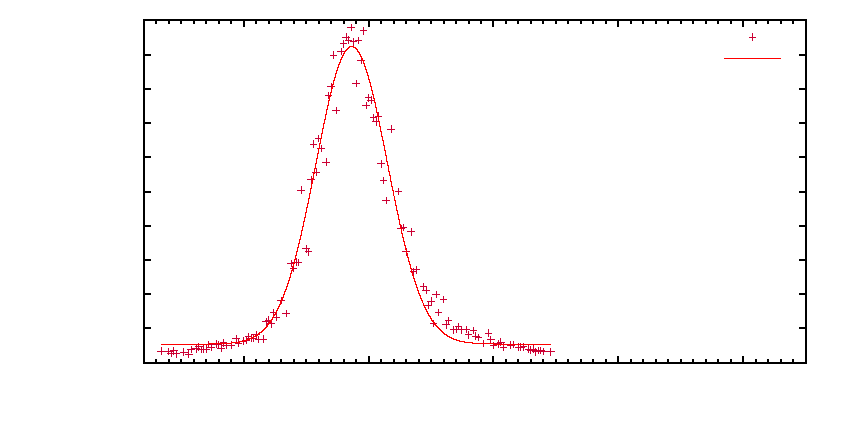
\includegraphics{linienscans_neues_schema_01_fake_AI_krass_mean}}%
    \gplfronttext
  \end{picture}%
\endgroup
